% Created 2021-05-13 Thu 20:49
% Intended LaTeX compiler: pdflatex
\documentclass[11pt]{article}
\usepackage[utf8]{inputenc}
\usepackage[T1]{fontenc}
\usepackage{graphicx}
\usepackage{grffile}
\usepackage{longtable}
\usepackage{wrapfig}
\usepackage{rotating}
\usepackage[normalem]{ulem}
\usepackage{amsmath}
\usepackage{textcomp}
\usepackage{amssymb}
\usepackage{capt-of}
\usepackage{hyperref}
\usepackage{minted}
\usepackage{tabularx}
\author{Philipp Beer}
\date{2021-05-10}
\title{Time Series Clustering: A Review}
\hypersetup{
 pdfauthor={Philipp Beer},
 pdftitle={Time Series Clustering: A Review},
 pdfkeywords={unic, 501dl, stassopoulou},
 pdfsubject={Literature review in time series clustering},
 pdfcreator={Emacs 27.2 (Org mode 9.4)}, 
 pdflang={English}}
\begin{document}

\maketitle




\section*{Time Series Clustering: A Review}
\label{sec:org5dcde06}
\url{https://552dlimages.s3-eu-west-1.amazonaws.com/unic\_logo.png}

Philipp Beer\\
Gradudate Program Data Science, UNIC\\
Prof. Athena Stassopoulou
\subsection*{Why you should listen to this talk}
\label{sec:org5b035e5}
If you want to \textbf{utilize time series} to create \textbf{forecasts},\\
\textbf{learn about their properties} or\\
\textbf{want to learn what is missing the research of time series clustering}\\
(IMHO) you should listen to this talk.
\subsection*{Introduction}
\label{sec:org4689d8c}
time series analysis an important part of machine learning

\subsubsection*{Applications}
\label{sec:org77858f6}
forecasting,\\
reporting,\\
analytics
\subsubsection*{Fields}
\label{sec:org12814ad}
natural sciences,\\
engineering,\\
finance,\\
medicine,\\
robotics
\subsubsection*{Challenges in time series analysis}
\label{sec:org59d6573}
\begin{itemize}
\item utilization of time series usually very challenging
\item many considerations required
\item oftentimes only limited set of historical data available
\end{itemize}
\subsubsection*{Time series clustering is used for}
\label{sec:org438f867}
Understand the intrinsic properties of time series oftentimes in context of adjacent time series
\subsubsection*{Focus of this review}
\label{sec:orgac5424e}
\begin{enumerate}
\item Definition  of terms clustering, time series and similarity measures
\item Clustering by what
\item Distance metrics
\item Clustering algorithms
\item Assessment
\item Limitations
\item Conclusion
\end{enumerate}

\subsection*{Definitions}
\label{sec:orgb0cbac9}
\subsubsection*{Clustering}
\label{sec:org4ee1ec0}
\begin{figure}[htbp]
\centering

\includegraphics[width=.9\linewidth]{./img/xray_vision.jpg}
\caption{1979 - The Health Education Council DC Comics}
\end{figure}
\begin{itemize}
\item \textbf{unsupervised} learning technique
\item reveal patterns useful for exploitations
\item segmentation, grouping, distinction of elements into groups
\end{itemize}
\subsubsection*{Time series}
\label{sec:org0133cdf}
\textbf{sequence composed by a series of continuous, real-valued elements}

\begin{itemize}
\item share the same challenges as high dimensional data
\item "curse of dimensionality"
\item quickly requires high computational power to process
\end{itemize}

\subsubsection*{Similarity measure in time series}
\label{sec:org97cdfd9}
\begin{itemize}
\item measure of how similar series are
\item usually computed pair-wise
\end{itemize}

\subsubsection*{Utility of Time series clustering}
\label{sec:org4e5416c}
anomalies, novelties, discord

\begin{itemize}
\item discover dynamic changes
\item generate predictions and recommendations
\item discover patterns
\end{itemize}

\subsection*{Clustering time series by}
\label{sec:org63e850f}
\subsubsection*{Shape-based clustering}
\label{sec:orgd8a8f04}
\begin{center}
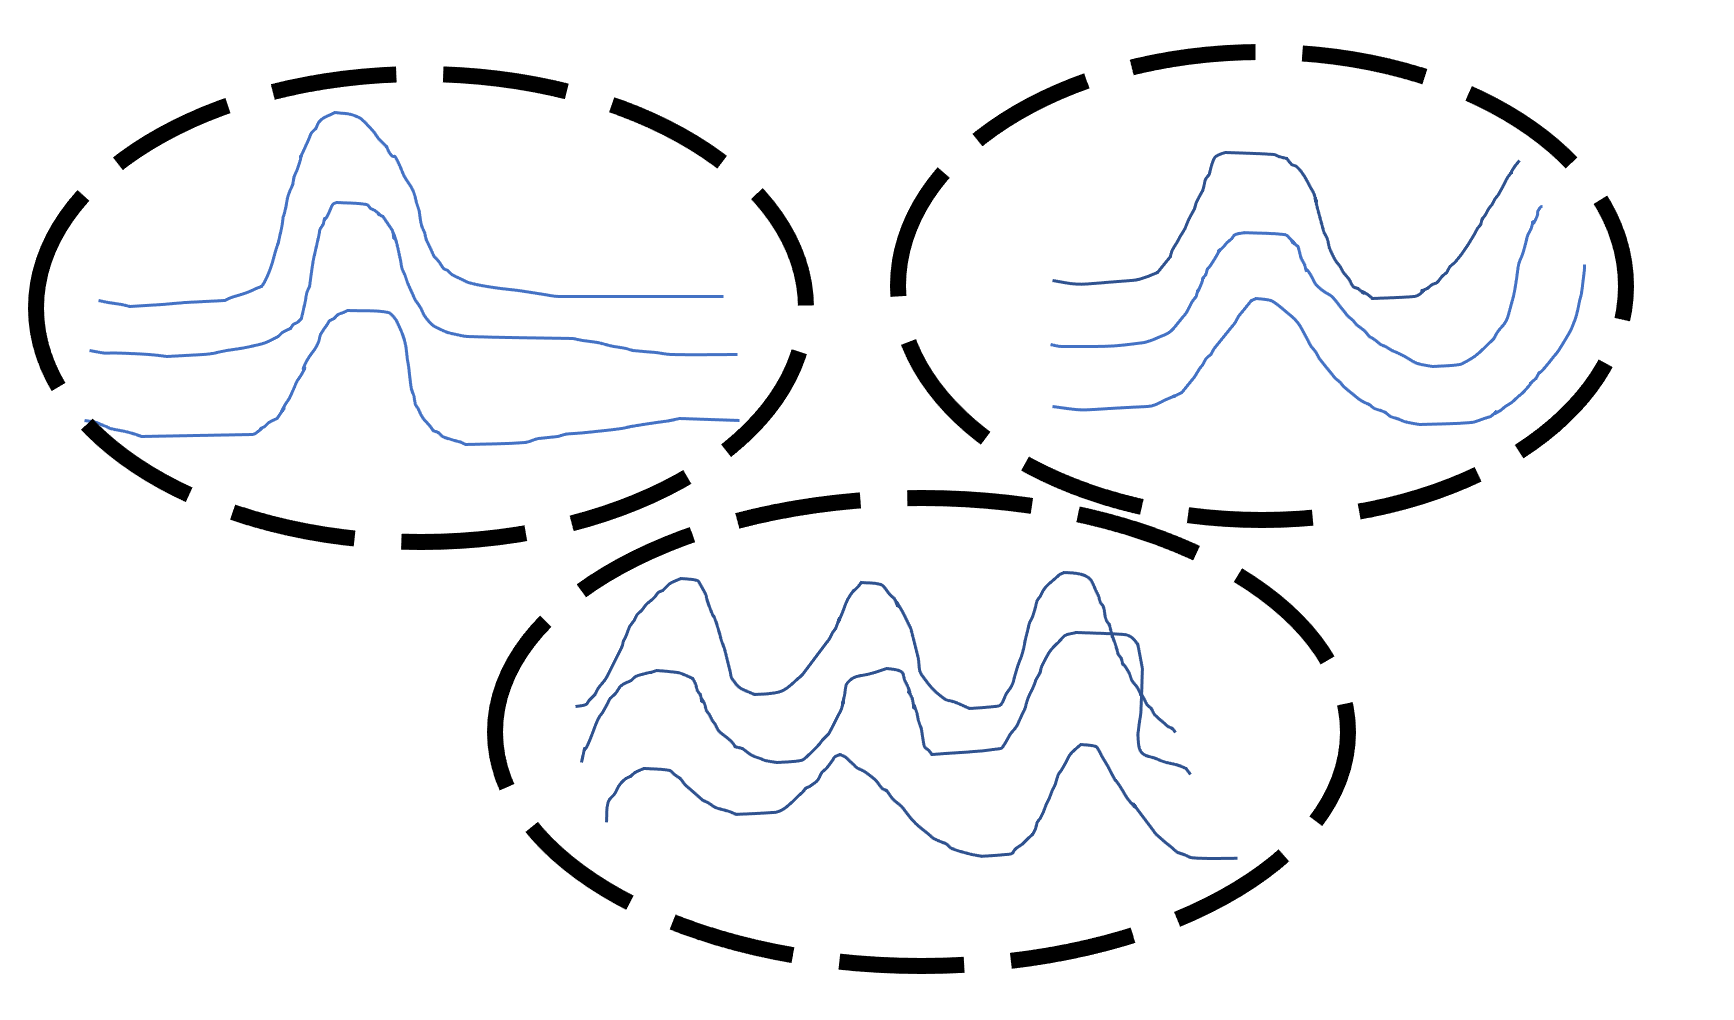
\includegraphics[width=.9\linewidth]{./img/shape_based_clustering.png}
\end{center}
\subsubsection*{Feature-based}
\label{sec:orgd85dcf4}
x
\begin{center}
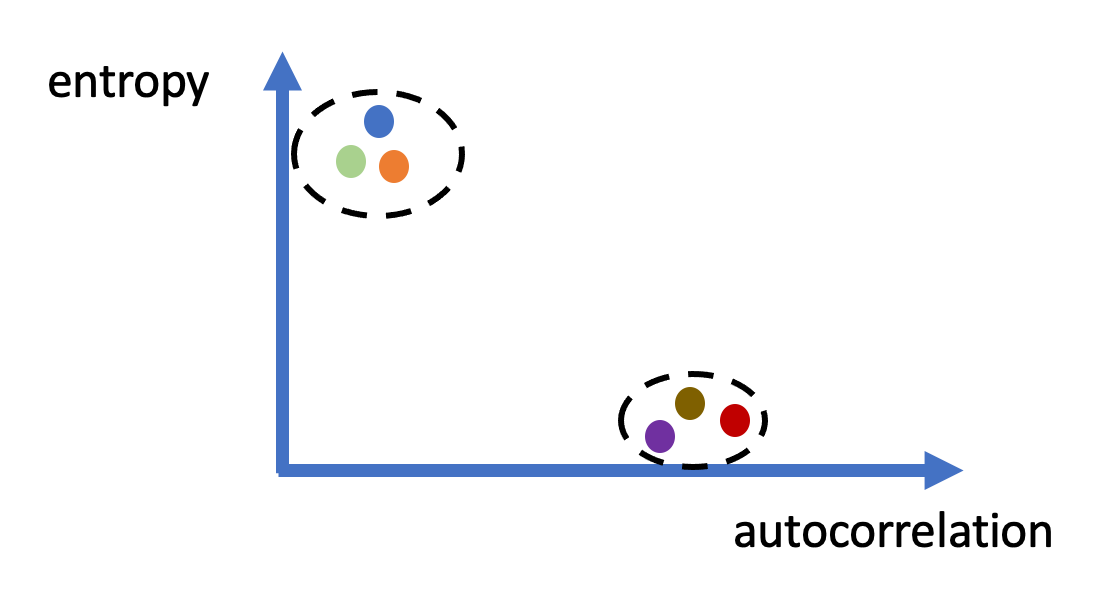
\includegraphics[width=.9\linewidth]{./img/feature_based_clustering.png}
\end{center}
\subsubsection*{Model-based}
\label{sec:orgcb8b761}
\begin{itemize}
\item transform raw time-series into model parameters
\item apply distance metric
\end{itemize}

\subsection*{Distance metrics}
\label{sec:orgf1b4e63}
\begin{itemize}
\item cornerstone of the clustering algorithm
\item depending on way of clustering chosen
\end{itemize}
\subsubsection*{stable distance metrics}
\label{sec:org7d06956}
dte.g. Euclidean distance
  $$ d(p,q) = \sqrt{(p_1 - q_1)^2 + \cdots + (p_n - q_n)^2} $$
\begin{itemize}
\item raw time series requires same length
\item no large outliers
\item limited noise
\end{itemize}
\begin{NOTES}
\begin{itemize}
\item Euclidean distance (ED) is very sensitive to unique features (outliers, noise)
\item ED requires same length time series
\end{itemize}
\end{NOTES}
\subsubsection*{approximate metrics}
\label{sec:orgdcf7c43}
\begin{center}
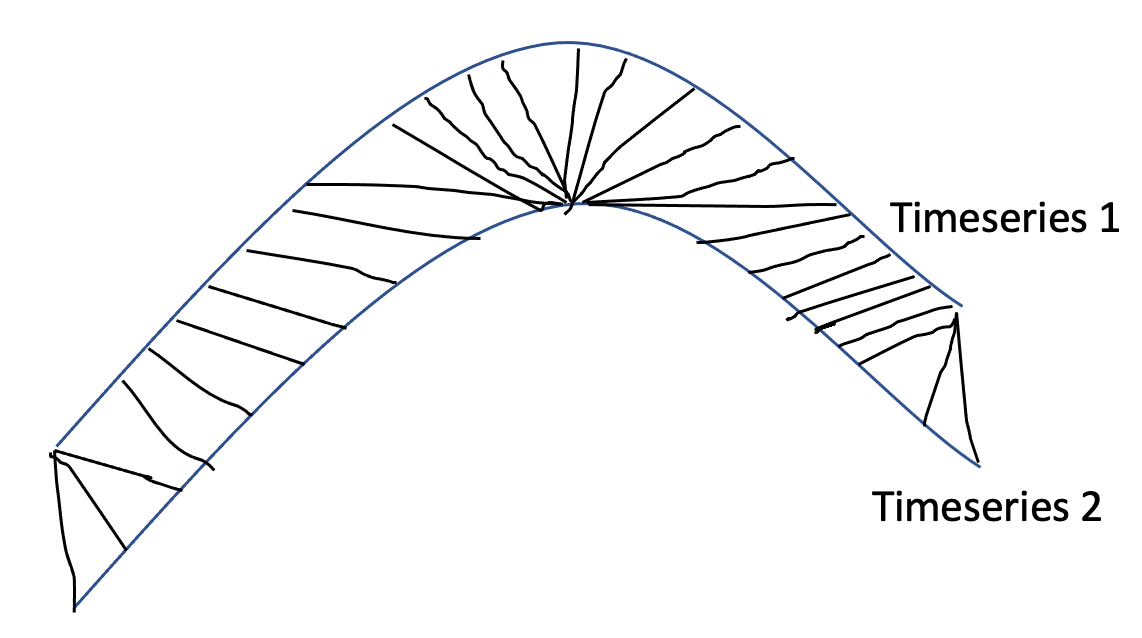
\includegraphics[width=500px]{./img/dtw_metric.png}
\end{center}
\begin{itemize}
\item can handle different length time series
\item Dynamic Time Warping (DTW)
\end{itemize}
\begin{NOTES}
\begin{itemize}
\item other metrics address part of these issues (e.g. DTW)
\item other methods introduce other issues (DTW - warping around local extremes)
\item complex methods often require parameters that can heavily impact performance (e.g. warping window)
\item more eloquent methods introduce high computational costs
\end{itemize}
\end{NOTES}

\subsubsection*{Current state of research}
\label{sec:org014d234}
\begin{itemize}
\item no existing framework how to choose these metrics
\item aim to identify new metrics or improve upon existing
\end{itemize}


\subsection*{Clustering algorithms}
\label{sec:org1b513c7}
\begin{table}[htbp]
\caption{\label{tab:org8b6b37d}Overview clustering algorithm types}
\centering
\begin{tabularx}{\columnwidth}{|l|X|}
\hline
Algorithm category & general description\\
\hline
Partional & aims to find prototype-based clusters and associates the time series with it; number of clusters is predefined (k)\\
\hline
Hierarchical & each time series starts as individual cluster and with iterations is associated with other time series to form a cluster by some measure of closeness\\
\hline
Density-based & associates time series into a cluster based on a density measure\\
\hline
Grid-based & quantizes feature space and segments time series into created intervals\\
\hline
\end{tabularx}
\end{table}

\subsubsection*{Partional}
\label{sec:org3ef80eb}
\begin{itemize}
\item grouping unlabeled data in groups
\item input parameter: \textbf{k}
\end{itemize}
\subsubsection*{Partional - crisp}
\label{sec:org98664df}
\begin{itemize}
\item K-Means / K-Medoids
\item utilizable with different distance metrics
\end{itemize}
\subsubsection*{Partional - fuzzy}
\label{sec:orgf88d424}
\begin{itemize}
\item fuzzy C-Keans / fuzzy K-Medoids
\item association to a cluster is defined by a probability
\item probabilities p of cluster associations:
$$ \sum{(p) = 1} $$
\end{itemize}
\subsubsection*{Hierarchical}
\label{sec:orgbb9e7a4}
\begin{center}
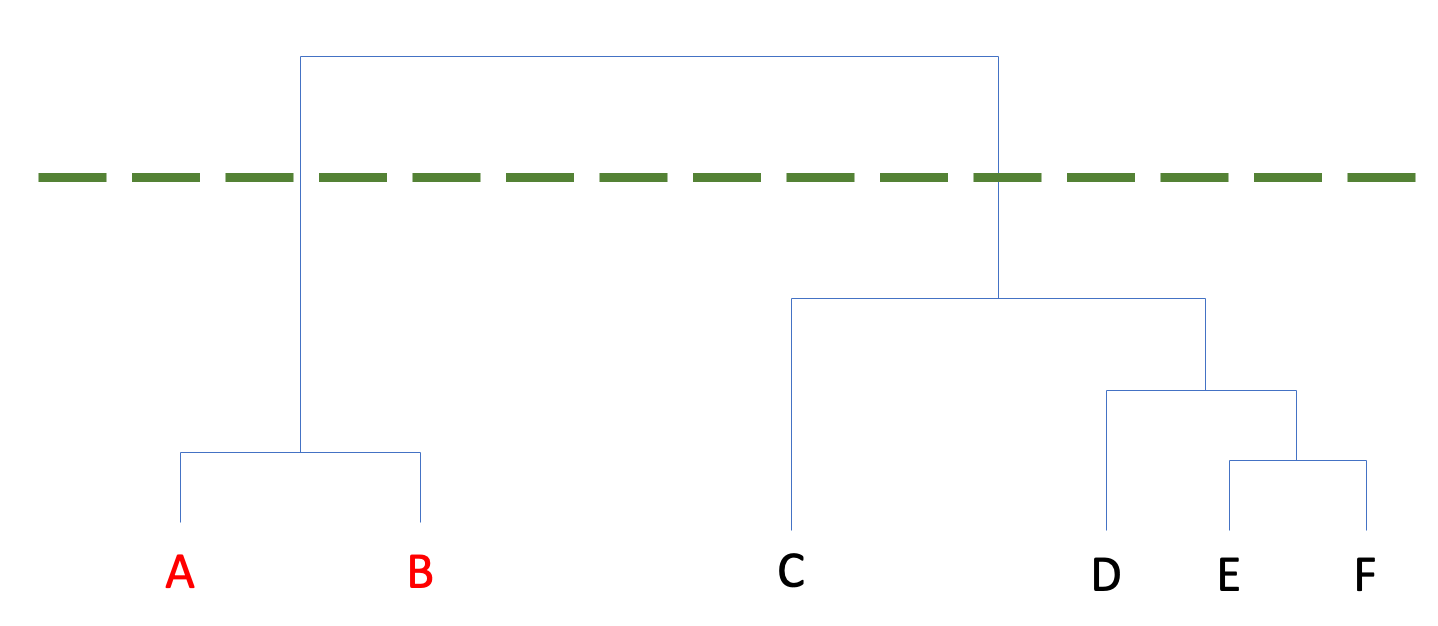
\includegraphics[width=.9\linewidth]{./img/dendogram.png}
\end{center}
\begin{itemize}
\item bottom-up and top-down approaches
\item distance measure: single-, average-, complete-link
\end{itemize}
\subsubsection*{Hierarchical - challenges}
\label{sec:orgca9d899}
\begin{itemize}
\item no adjustments after decision about an element made
\item computational complexity: $$ \mathcal{O}(N^2) $$
\end{itemize}
\subsubsection*{Hierarchical - advantages}
\label{sec:orgd7db302}
\begin{itemize}
\item visual analysis
\item no predetermination of k required
\end{itemize}

\subsubsection*{Grid-based methods}
\label{sec:org47325a7}
\begin{center}
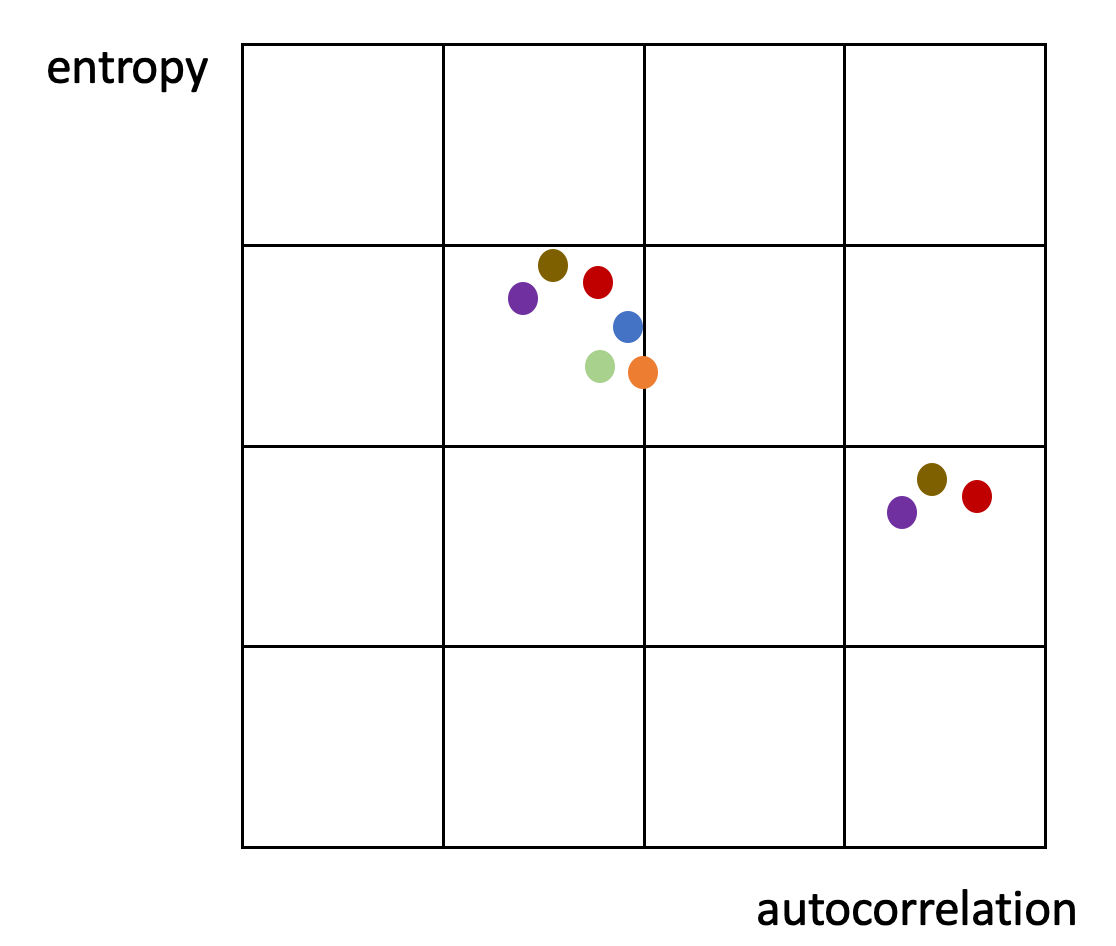
\includegraphics[width=.9\linewidth]{./img/grid_based.png}
\end{center}
\begin{itemize}
\item quantizing the feature space into hyper-rectangles (cells)
\item for reach range of those intervals the respective metrics are computed
\end{itemize}
\begin{itemize}
\item Challenges
\label{sec:orgeda1bf8}
\begin{itemize}
\item no relationship between the grids is created
\item interval range is a manual parameter and not inherent of the algorithm
\item question: Can these ranges be inferred from the data?
\end{itemize}
\item Advantages
\label{sec:orgf446c72}
\begin{itemize}
\item single pass computation $$ \mathcal{O}(N) $$
\item very fast query impacted only by number of grids (k): \$\$ \mathcal
\end{itemize}
\end{itemize}
\subsubsection*{Density-based methods}
\label{sec:orgf60ddce}
\begin{itemize}
\item DBSCAN
\item two parameters (neighbourhood and minimum for points)
\end{itemize}
\begin{itemize}
\item Challenges
\label{sec:orga26ad2e}
\begin{itemize}
\item correct setup of parameters requires higher understanding of the data
\item varying cluster densities create a challenge
\item not often applied in time series due to this complexity
\end{itemize}
\item Advantages
\label{sec:org6e33770}
\begin{itemize}
\item can handle non-globular shapes well
\item quick execution speed
\item is capable of identifying noise and outliers
\item those properties make it applicable to a wide variety of data sets
\end{itemize}
\end{itemize}

\subsection*{Assessment metrics}
\label{sec:org6162d3c}
\subsubsection*{General points}
\label{sec:org25ed068}
\begin{itemize}
\item assessment is the trickiest part of the process
\item metrics are separated into \textbf{external} and \textbf{internal} metrics
\item implementations usually contain experimental flaws (data and implementation bias)
\item limits the generalizability of study results to real-world problems
\end{itemize}
\subsubsection*{Solution proposals}
\label{sec:org1c1c1fa}
\begin{itemize}
\item always test implementation on a wide variety of data to verify (e.g. M4)
\item compare novel similarity measures to established ones
\end{itemize}
\subsubsection*{Assessment with respect to what (IMPORTANT)}
\label{sec:org3297859}
\begin{itemize}
\item usually subsequent analytical step determines the value of the chosen clusters
\item pre-determined clusters are also only a specific usage of the underlying data
\end{itemize}
\subsubsection*{External indexes}
\label{sec:orgec34744}
\begin{itemize}
\item validation of clusters that exist outside of algorithm (often ground truth)
\item degree of matching between two partitions
\item Cluster Purity, Rand Index, F-measure, Entropy, Jaccard index
\end{itemize}
\subsubsection*{Internal indexes}
\label{sec:orgee54541}
\begin{itemize}
\item evaluation of a goodness of clustered structure
\item core idea: elements of same cluster close together / elements of other clusters well separated
\item Sum of Squared Errors, Silhouette score, R\textsuperscript{2} index, \ldots{}
\end{itemize}

\subsection*{Limitations}
\label{sec:org4608330}
\subsubsection*{General}
\label{sec:orgc81e167}
\begin{itemize}
\item generally clustering algorithms do not perform well with time series
\item dimensionality, noise and the dynamic nature of time series are problematic
\item dimensionality reduction inherently brings \textbf{information loss}
\item research in this field is primarily focused on univariate time series
\item limited scope of time series are used for time series clustering research
\end{itemize}
\subsubsection*{Representation methods}
\label{sec:org45bc2df}
\begin{itemize}
\item data-adaptive and model-based representation reduces dimensionality but struggles with the analysis of multiple series
\item non-data-adaptive methods struggle with variying length time series.
\end{itemize}
\subsubsection*{Simlarity metrics}
\label{sec:org250c073}
\begin{itemize}
\item no framework for choosing appropriate distance metric exists
\item the user needs to choose between generally sensitive metrics (e.g. ED) and computationally expensive metrics (e.g. DTW)
\item additionally very few metrics exceed the ED performance
\end{itemize}
\subsubsection*{Algorithms}
\label{sec:org1b15ea2}
\begin{itemize}
\item popular methods like K-Means, K-Medoids struggle with non-globular shapes (property that is visually not observable in high-dimensional data) and are negatively impacted by outliers and noise
\item having to define parameters of algorithms in part is counter to the idea of learning patterns from the data without input
\item other algorithm categories address these issues at the price of computational complexity and infeasibility for large data sets
\end{itemize}
\subsection*{Conclusions and things you should remember}
\label{sec:org830c20d}
\begin{itemize}
\item no clear pattern emerged which methods and metrics are to be used in which circumstances, likely due to lack of generalizability of the found results
\item adding complexity to current research may not serve the goals of finding meaningful algorithms and methods any more than already did
\item our proposal: focus research efforts more on finding fundamental truths about this process
\begin{itemize}
\item when to use/avoid certain metrics or algorithms
\item clarity here: may improve general understanding
\end{itemize}
\end{itemize}
\subsection*{Thank you. Which questions do you have?}
\label{sec:orgb99882d}
\end{document}